\section{Evaluations and Experimental Design}

\textit{Formative} early in the design process, sanity checks that we're building the right thing. \textit{Summative} to check if we improved upon our last iteration, does it work better than other solutions? \medskip

\textbf{Quantitative Evaluation Methods}

Ensure certain level of quality, comparesolutions objectively, attain a scientific statement. \medskip

\textbf{Primary Usability Metrics} \smallskip

\begin{center}
	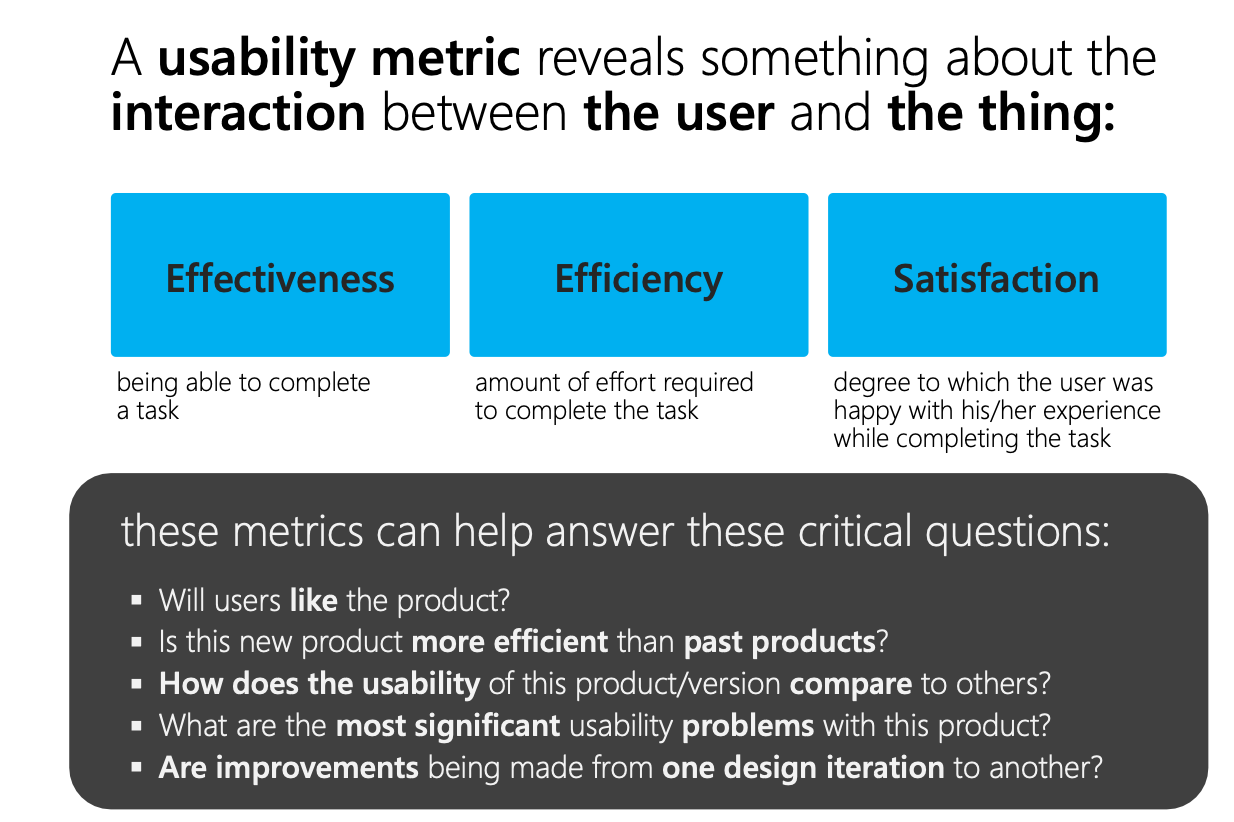
\includegraphics[width=\linewidth]{metrics.png}
\end{center}

\textbf{Cause and Effect} \smallskip

We want to identify clear causal links. Cause precedes effect, they need to correlate and other explanations have to be ruled out. 
Isolate causality by controlled experiments. Alter design with suspected cause absent (control) and present (experimental condition).
All other conditions should be identical. \medskip

\textbf{Quasiexperimentell | Observational} \smallskip

We observe that independent variable and dependent variable are highly correlated, but did not control for anything (for instance participation in exercices and final exam grade). \medskip

\textbf{Experimental | Controlled} \smallskip

We randomly assign students to exercise and no exercise condition, then we controlled for other variables and results implies causality. \medskip


\textbf{characteristics of Emprical Methods}

\begin{itemize}
    \item Objectivity
    \item Reproducibility
    \item Validity (internally and externally)
    \item Relevance
\end{itemize}

For instance threat to external validity is over-use of specific participant groups (only psychology or cs students). \medskip

\textbf{The experiment}

Indepdendent variables affect the dependent (measured) variables through experiment.

Variables can be catagorical, ordinal (ordered discrete), or cardinal/interval (continuous) data. \medskip

\textbf{Designing an empirical study}

\begin{enumerate}
    \item What is being compared? (which Indepdendent variables)
    \item What are they bing comapred in? (dependent variables, metrics)
    \item What lse is being varied? (extraneous variables to control/eliminate)
    \item Relevance
\end{enumerate}

Look at slide set 5 for various examples. \medskip

\textbf{More complex comparisons}

Different experimental designs possible: \textit{Within subjects:} Everyone-does everything. \textit{Between subjects:} Only on condition per group. \medskip

\textbf{Latin Square Counterbalancing}

\begin{center}
	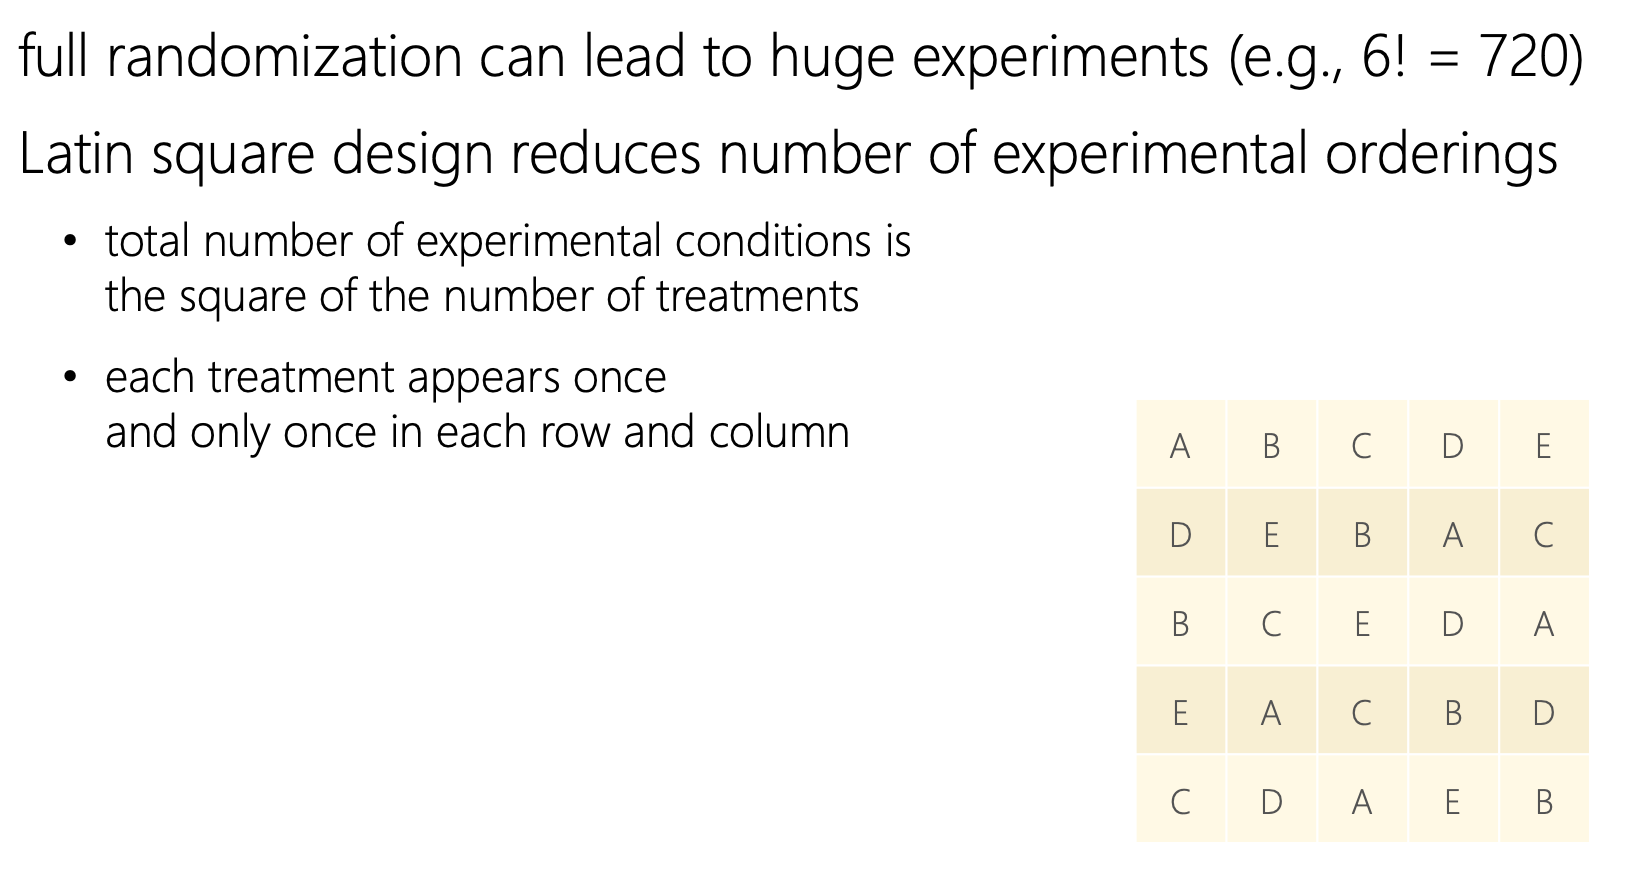
\includegraphics[width=\linewidth]{latin_square.png}
\end{center}


\textbf{Latin Square Example for 5}

\begin{center}
	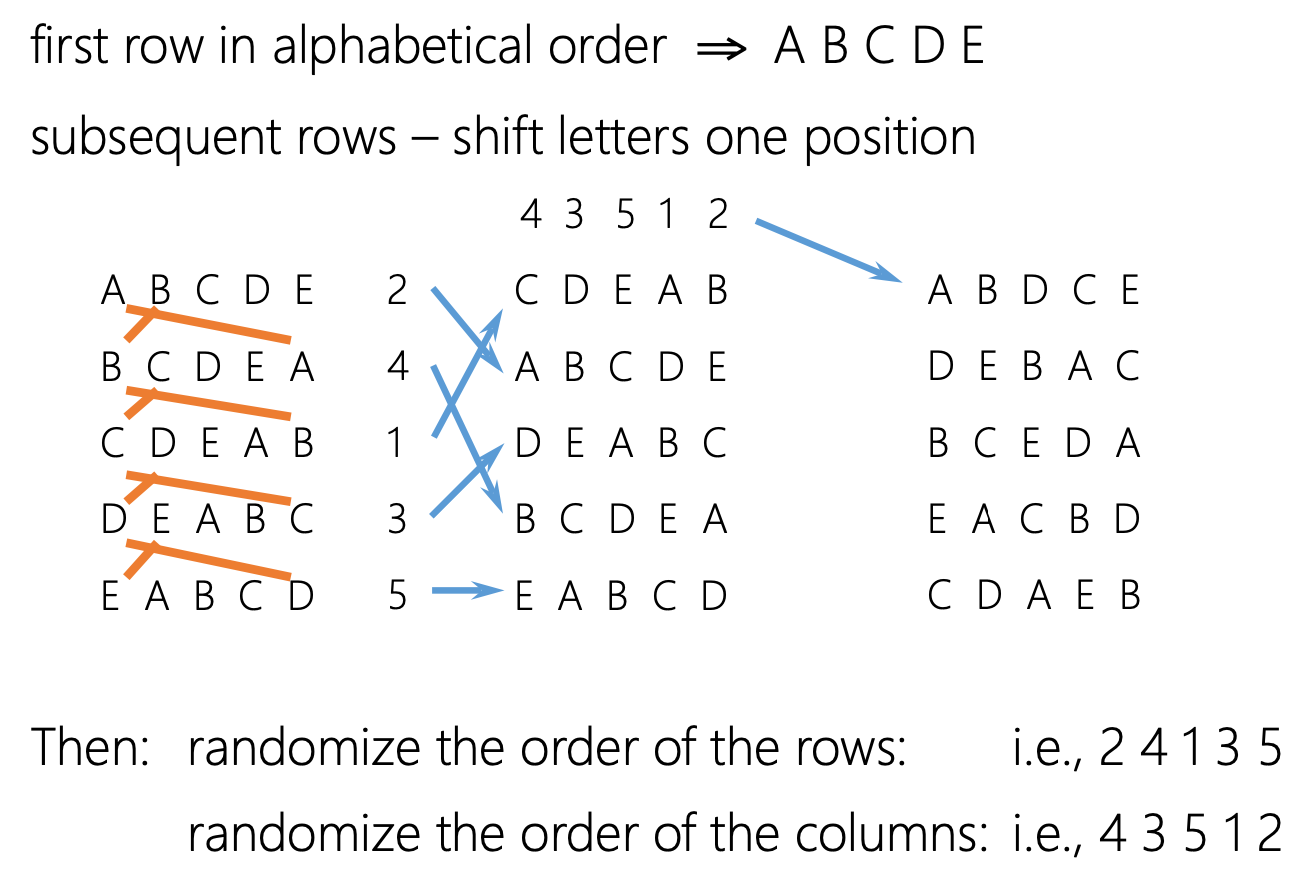
\includegraphics[width=\linewidth]{latin_example.png}
\end{center}